\documentclass[border=5pt]{standalone}
\usepackage{helvet}
\renewcommand{\familydefault}{\sfdefault}
\usepackage{tikz}
\usepackage{amsmath}
\usetikzlibrary{positioning,arrows.meta,fit,backgrounds,calc}

\begin{document}
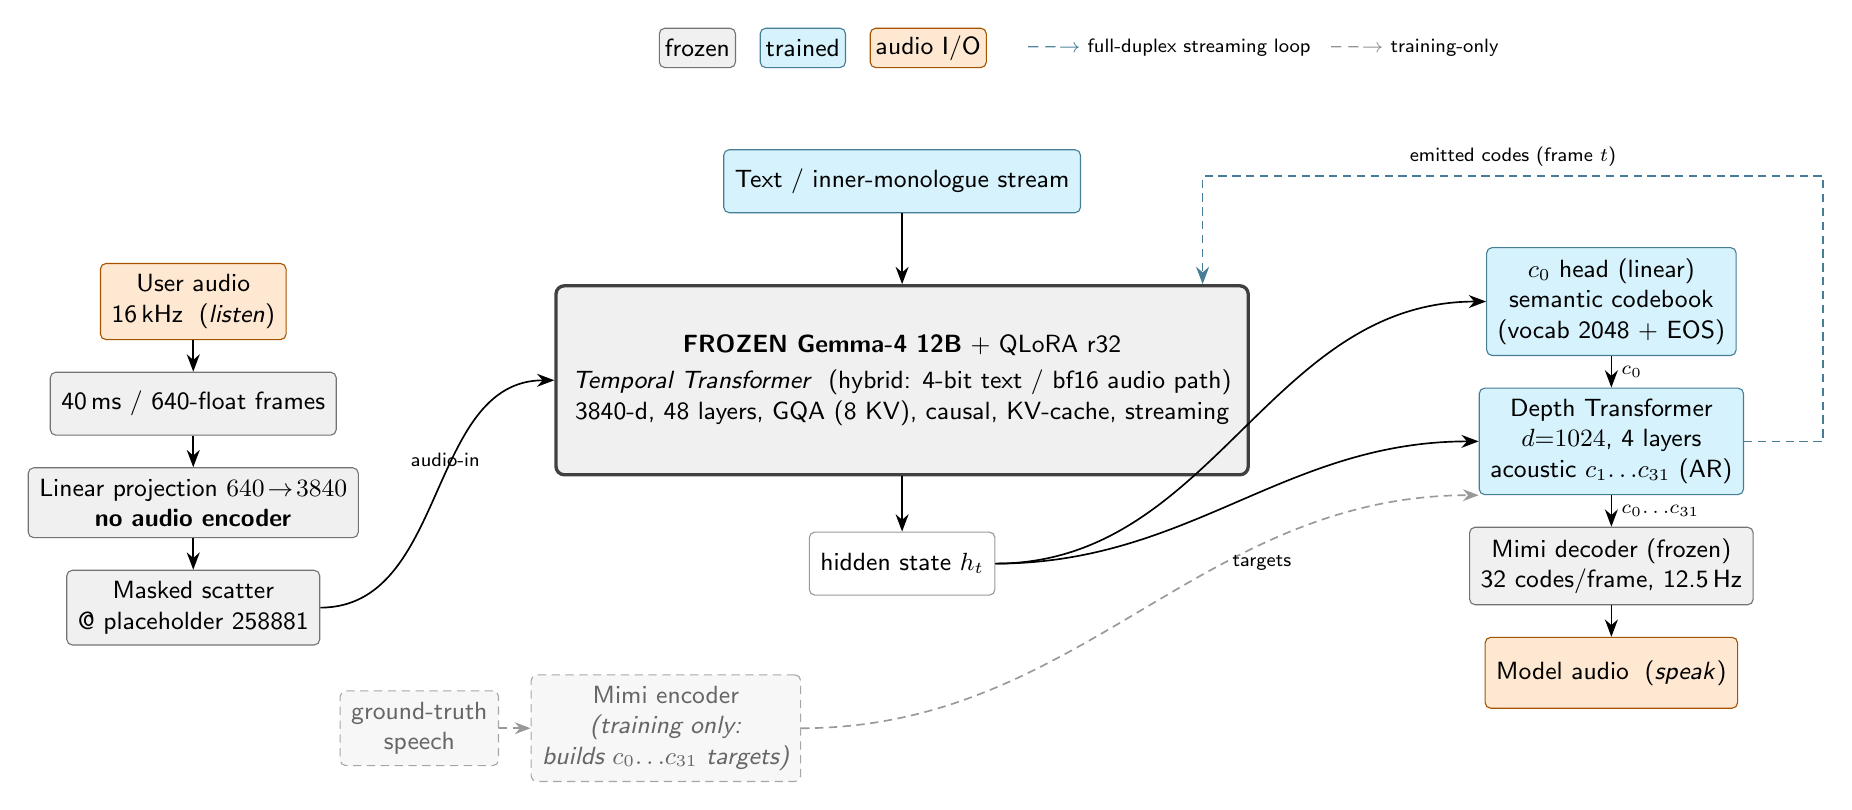
\begin{tikzpicture}[
  font=\small,
  box/.style={rectangle, rounded corners=2pt, draw=black!55, align=center,
              inner sep=4pt, minimum height=8mm},
  frozen/.style={box, fill=gray!12},
  trained/.style={box, fill=cyan!16, draw=cyan!55!black},
  io/.style={box, fill=orange!18, draw=orange!65!black, minimum height=9mm},
  train_only/.style={box, fill=gray!6, draw=black!35, densely dashed, text=black!60},
  bb/.style={rectangle, rounded corners=3pt, draw=black!75, very thick,
             fill=gray!12, align=center, inner sep=6pt,
             minimum width=70mm, minimum height=24mm},
  arr/.style={-{Stealth[length=2.2mm]}, semithick},
  loop/.style={-{Stealth[length=2.2mm]}, semithick, densely dashed, draw=cyan!55!black},
  trainarr/.style={-{Stealth[length=2mm]}, semithick, densely dashed, draw=black!40},
]

% ---------- BACKBONE (center) ----------
\node[bb] (bb) {\textbf{FROZEN Gemma-4 12B} $+$ QLoRA r32\\[2pt]
  \emph{Temporal Transformer} \;(hybrid: 4-bit text / bf16 audio path)\\
  3840-d, 48 layers, GQA (8 KV), causal, KV-cache, streaming};

% ---------- LISTEN path (left, encoder-free) ----------
\node[io, left=34mm of bb.west, anchor=east, yshift=10mm] (mic) {User audio\\16\,kHz \;(\emph{listen})};
\node[frozen, below=4mm of mic] (frames) {40\,ms / 640-float frames};
\node[frozen, below=4mm of frames] (proj) {Linear projection $640\!\to\!3840$\\\textbf{no audio encoder}};
\node[frozen, below=4mm of proj] (scat) {Masked scatter\\@ placeholder 258881};

\draw[arr] (mic) -- (frames);
\draw[arr] (frames) -- (proj);
\draw[arr] (proj) -- (scat);
\draw[arr] (scat.east) to[out=0,in=180] node[above,font=\scriptsize,pos=0.55]{audio-in} (bb.west);

% ---------- TEXT stream (top) ----------
\node[trained, above=9mm of bb] (txt) {Text / inner-monologue stream};
\draw[arr] (txt) -- (bb.north);

% ---------- hidden state ----------
\node[box, fill=white, draw=black!40, below=7mm of bb] (h) {hidden state $h_t$};
\draw[arr] (bb.south) -- (h);

% ---------- SPEAK path (right / down, Mimi-code head) ----------
\node[trained, right=30mm of bb.east, anchor=west, yshift=10mm] (c0) {$c_0$ head (linear)\\semantic codebook\\(vocab 2048 $+$ EOS)};
\node[trained, below=4mm of c0] (depth) {Depth Transformer\\$d{=}1024$, 4 layers\\acoustic $c_1\!\dots\!c_{31}$ (AR)};
\node[frozen, below=4mm of depth] (mdec) {Mimi decoder (frozen)\\32 codes/frame, 12.5\,Hz};
\node[io, below=4mm of mdec] (spk) {Model audio \;(\emph{speak})};

\draw[arr] (h.east) to[out=0,in=180] (c0.west);
\draw[arr] (h.east) to[out=0,in=180] (depth.west);
\draw[arr] (c0) -- node[right,font=\scriptsize]{$c_0$} (depth);
\draw[arr] (depth) -- node[right,font=\scriptsize]{$c_0\!\dots\!c_{31}$} (mdec);
\draw[arr] (mdec) -- (spk);

% feedback: emitted codes embed back as audio-out input next frame
% routed as a clean right-angle loop over the top, clear of all boxes
\coordinate (laneX)  at ($(c0.east)+(11mm,0)$);
\coordinate (fbTopY) at ($(c0.north)+(0,9mm)$);
\coordinate (fbP1)   at (laneX |- depth.east);
\coordinate (fbP2)   at (laneX |- fbTopY);
\coordinate (bbTop)  at ($(bb.north east)+(-6mm,0)$);
\coordinate (fbP3)   at (bbTop |- fbTopY);
\draw[loop] (depth.east) -- (fbP1) -- (fbP2)
   -- node[above,font=\scriptsize,align=center,pos=0.5]{emitted codes (frame $t$)} (fbP3)
   -- (bbTop);

% ---------- training-only Mimi encoder ----------
\node[train_only, below=10mm of h, xshift=-30mm] (menc) {Mimi encoder\\\textit{(training only:}\\\textit{builds $c_0\!\dots\!c_{31}$ targets)}};
\node[train_only, left=4mm of menc] (gt) {ground-truth\\speech};
\draw[trainarr] (gt) -- (menc);
\draw[trainarr] (menc.east) to[out=0,in=180] node[below,font=\scriptsize,pos=0.7]{targets} (depth.south west);

% ---------- legend ----------
\begin{scope}[shift={($(bb.north)+(-26mm,30mm)$)}]
  \node[frozen, minimum height=5mm, inner sep=2pt] (l1) {frozen};
  \node[trained, minimum height=5mm, inner sep=2pt, right=3mm of l1] (l2) {trained};
  \node[io, minimum height=5mm, inner sep=2pt, right=3mm of l2] (l3) {audio I/O};
  \node[right=4mm of l3, font=\scriptsize, align=left] (l4)
    {{\color{cyan!55!black}-- -- $\!\to$} full-duplex streaming loop\quad
     {\color{black!45}-- -- $\!\to$} training-only};
\end{scope}

\end{tikzpicture}
\end{document}
